\chapter{Motivation: The Long-Context Memory Wall}
\label{ch:motivation}

The motivation in this chapter comes from the checked-in traces rather than from a generic claim that ``memory matters.'' In the short-context runs, dense compute is still visible enough that a faster matrix engine would help. In the long-context runs, the historical KV reads become the dominant term, and the useful decode rate is set by how quickly the memory system can revisit old tokens. I use that change in the trace profile to derive the requirements used in the two design chapters.

\section{The KV Cache Capacity and Bandwidth Crisis}

During decode, every new token consults the KV entries produced by prefill and by earlier decode iterations. The storage footprint grows one token at a time, while the read pressure is paid repeatedly at generation time. That asymmetry is what makes the cache more than a capacity bookkeeping problem.

\begin{figure}[htbp]
\centering
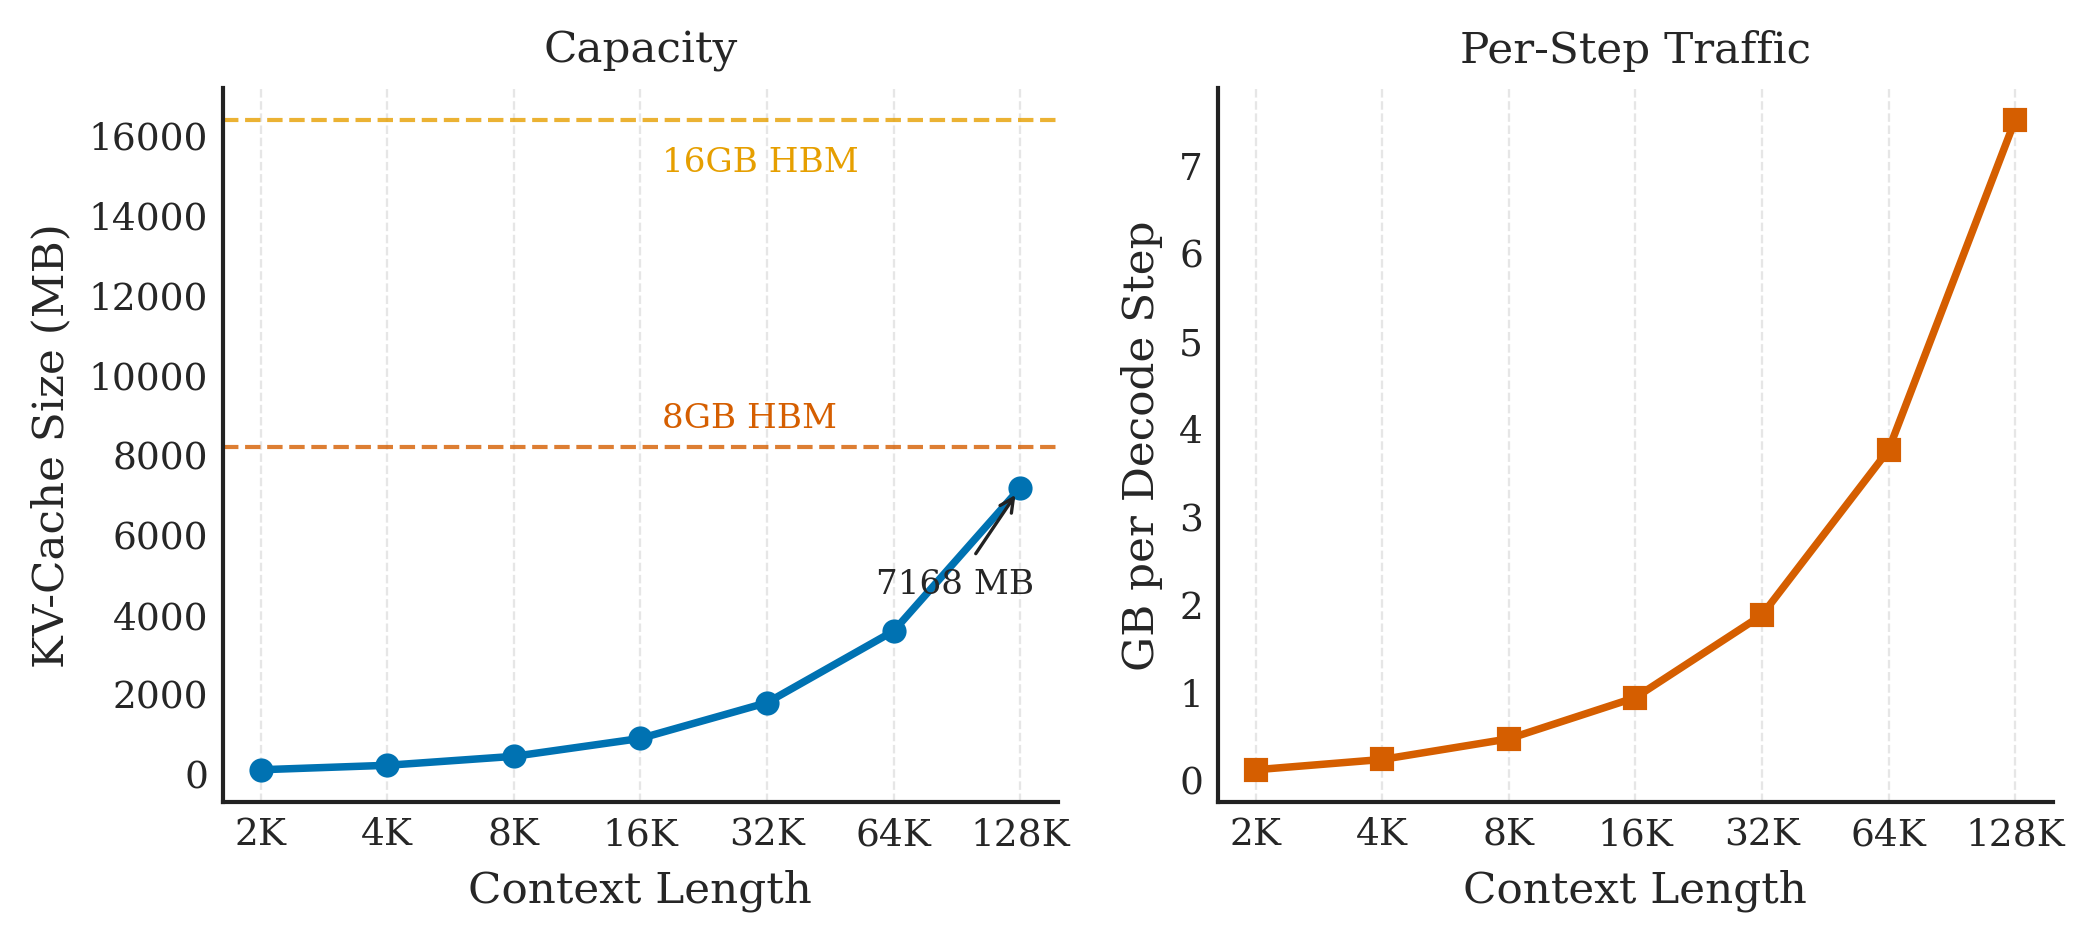
\includegraphics[width=\textwidth]{../paper_assets/figures/fig3_kv_cache_scaling.png}
\caption[KV-cache scaling with context length]{KV-cache processing scale factor as the sequence length approaches long-context settings without out-of-memory failures.}
\label{fig:scaling}
\end{figure}

Figure~\ref{fig:scaling} uses a Qwen2.5-7B-style configuration to show the scale of the state. With 28 layers, four grouped-query KV heads, 128 dimensions per head, and FP16 storage, one $128{,}000$-token request requires more than 7\,GB of KV-cache space~\cite{vllm}. That is already a large allocation for one user; under batching or multi-tenant serving, the same linear term quickly consumes the memory budget that would otherwise hold additional requests.

The same trend can be written as a simple per-token footprint. For the evaluated grouped-query configuration, each token contributes:
\begin{equation}
2 \times 28 \times 4 \times 128 \times 2 = 57{,}344 \ \text{bytes}
\end{equation}
where the leading factor of two accounts for keys and values. Table~\ref{tab:kv_footprint} expands this value across the context lengths used in the experiments. The table is useful because it separates capacity pressure from bandwidth pressure: the memory system must reserve the footprint once, but it must revisit the stored history during every decode step.

\begin{table}[htbp]
\centering
\caption[KV-cache footprint across context lengths]{Bytes reserved by one request in the Qwen2.5-7B-style trace; values follow from the grouped-query layout above.}
\label{tab:kv_footprint}
\begin{tabular}{lrr}
\toprule
\textbf{Context Length} & \textbf{Bytes per Request} & \textbf{Approx. Size} \\
\midrule
2K   & 117,440,512   & 112 MiB \\
8K   & 469,762,048   & 448 MiB \\
32K  & 1,879,048,192 & 1.75 GiB \\
64K  & 3,758,096,384 & 3.50 GiB \\
128K & 7,340,032,000 & 6.84 GiB \\
\bottomrule
\end{tabular}
\end{table}

CXL can provide the required capacity, but the traffic requirement remains severe. A decode stream that emits 20 tokens/s and repeatedly revisits multi-gigabyte historical state can quickly approach the practical bandwidth of a PCIe/CXL link~\cite{direct_cxl}. This is why the later designs treat long-context serving as both a placement problem and a movement problem.

\section{Latency Profiling}

The per-token profile is divided into three terms. The first term is model arithmetic on weights and the current hidden state. The second is format work, including unpacking or conversion when compressed integer state is consumed by a higher-precision compute path. The third is historical KV access, which covers movement and memory service time for keys and values generated by earlier tokens.

\begin{figure}[htbp]
\centering
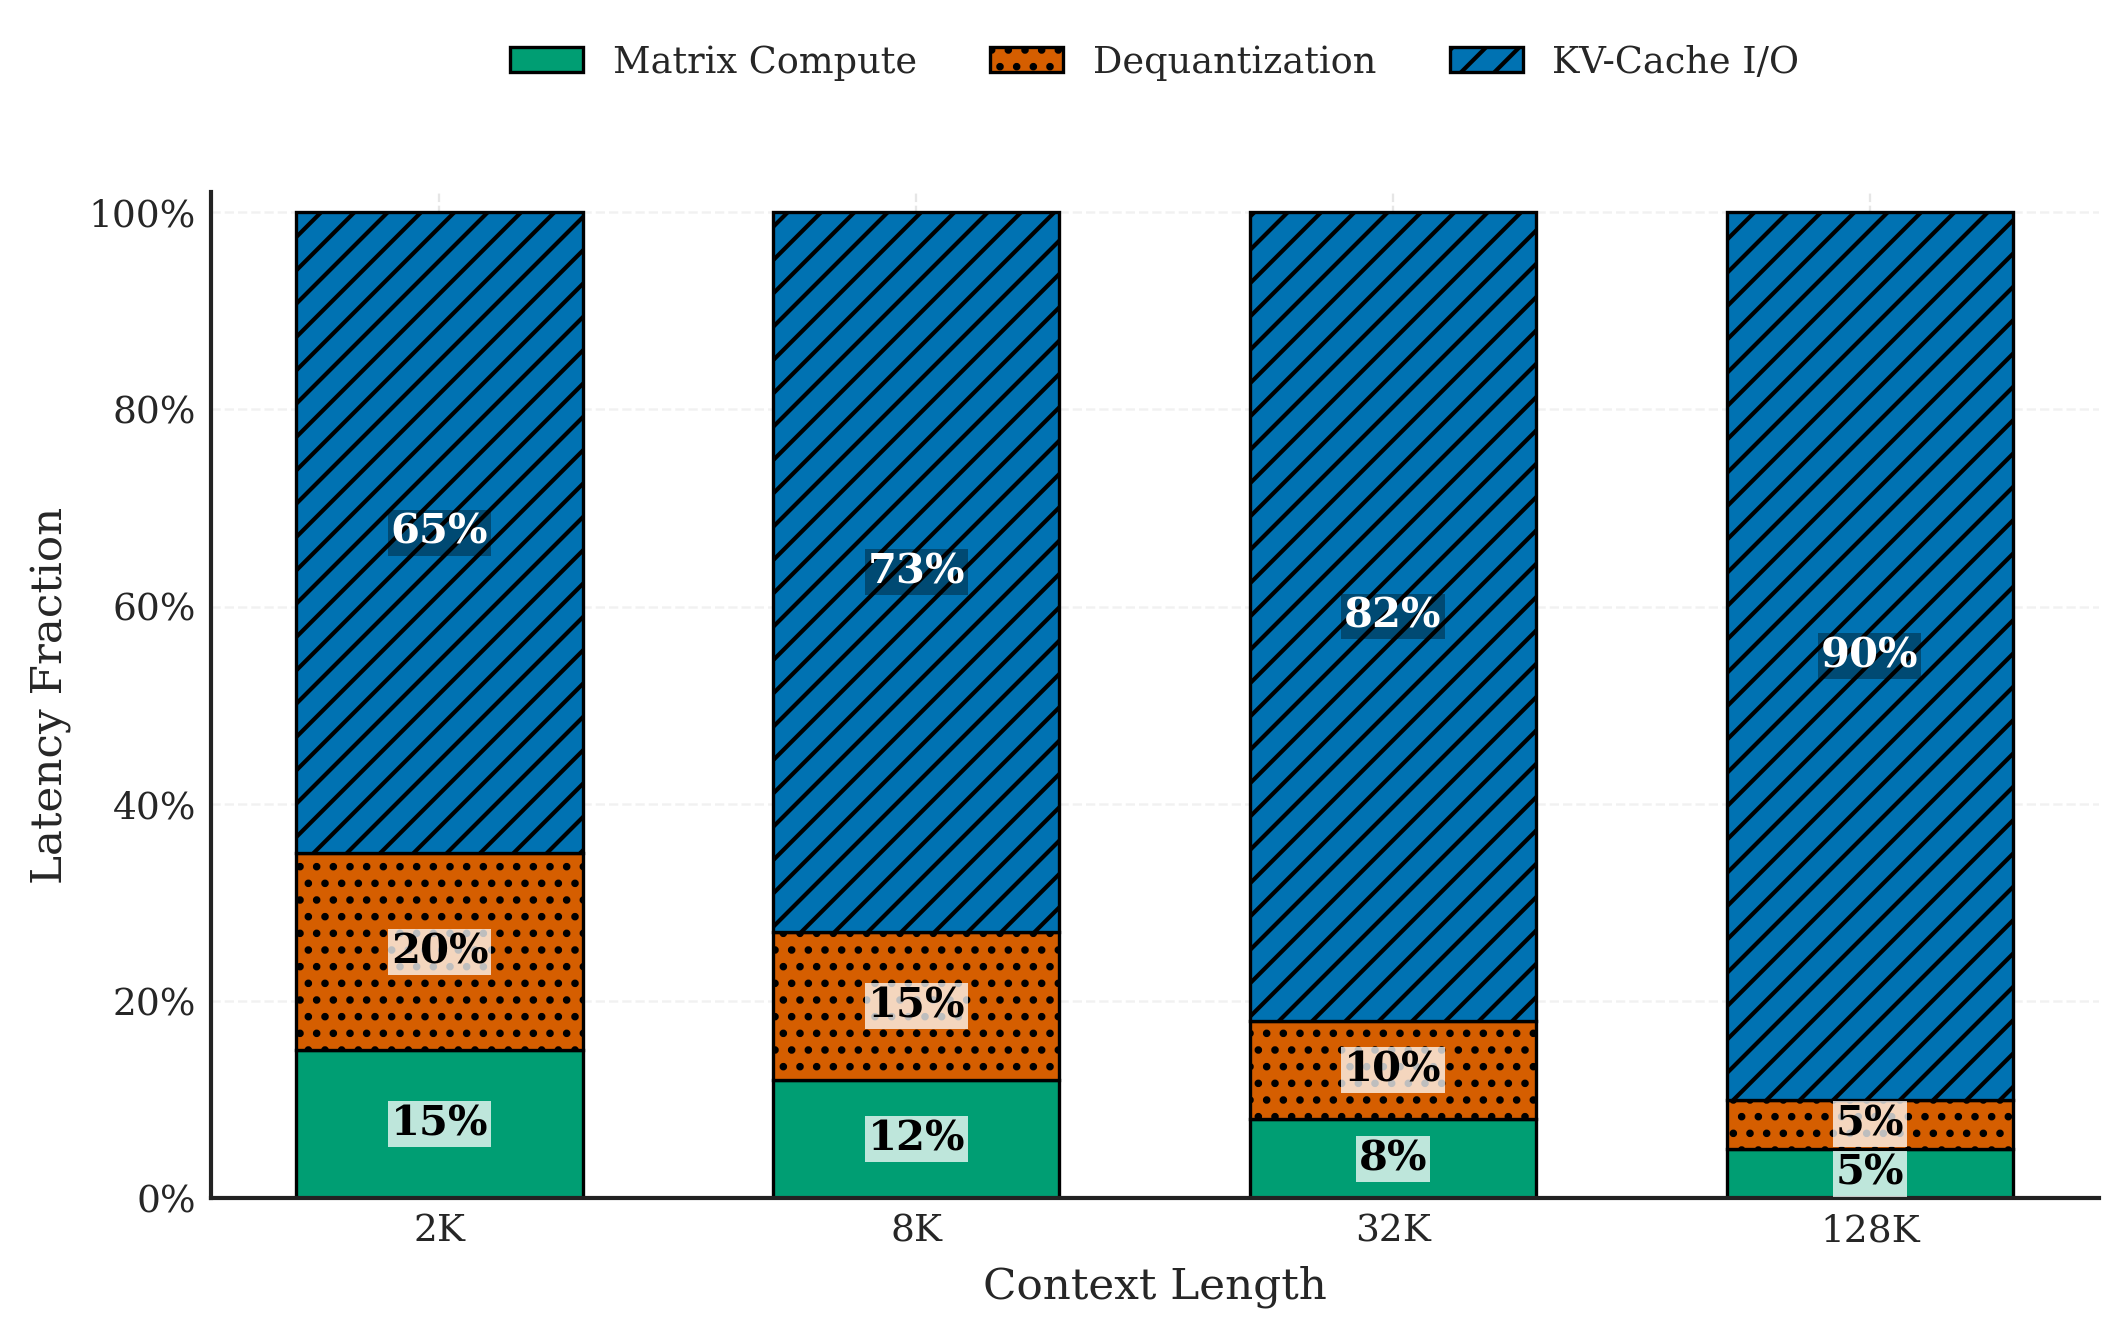
\includegraphics[width=\textwidth]{../paper_assets/figures/fig1_latency_breakdown.png}
\caption[Latency breakdown across context lengths]{Profiler output used to choose design targets, with arithmetic, conversion, and old-token KV service shown separately.}
\label{fig:latency}
\end{figure}

Figure~\ref{fig:latency} shows where the crossover occurs. At 2K and 8K contexts, model arithmetic still occupies a visible part of the total. At 32K and 128K contexts, the bar is mostly historical KV traversal, with format conversion still large enough to matter. I therefore use the profile as a guide for the rest of the design: improving the matrix engine alone would miss the term that grows fastest.

\subsection{The Reality of PIM Format Mismatches}

Moving attention closer to the KV cache addresses only half of the profile. The other half is numeric format. Practical serving stacks often store KV-cache tensors in low precision, for example INT8, to stretch memory capacity~\cite{llm_outliers}. Existing memory-proximate compute engines commonly provide floating-point softmax or other wide nonlinear datapaths~\cite{pim_quant}. If the PIM pipeline has to unpack integer KV data, evaluate the nonlinear stage in floating point, and then repack the result, a significant part of the near-memory advantage is lost to conversion.

\section{Summary}

The evidence in this chapter leaves two design requirements. First, the largest repeated object in the decode loop should not be dragged back to the host whenever a token is generated. Second, the nonlinear portion of attention should not force the cache to leave its compact representation before any useful near-memory work happens. LKC-CXL-PIM addresses these requirements inside one endpoint, and DisaggKV tests the same principles when the cache is spread across a CXL pool.

These requirements become the design checklist used in the next two chapters:
\begin{enumerate}
    \item \textbf{Move work to the cache rather than moving the cache to the host.} The historical KV cache is the repeated state object in long-context decode, so the architecture should minimize host-facing transfers of that state.
    \item \textbf{Keep the common case narrow.} Quantized KV-cache storage is only useful if the memory-side datapath can consume it without expanding ordinary activations into a floating-point pipeline.
    \item \textbf{Synchronize only what must be global.} Distributed attention needs a shared maximum and sum for correct softmax normalization. Those values are scalars, so the multi-node design treats scalar reduction as the natural CXL fabric primitive.
\end{enumerate}
